\section{Analysis}\label{sec:analysis}
In this section we analyse different aspects of the simulations. In Section \ref{sec:description} we describe the simulations, their underlying models and give an overview of their properties. The next step in Section \ref{sec:cmd_plots} is to fit isochrones to the \ac{CMD} to verify given age and metallicity. After that, we investigate the phase space in Section \ref{sec:phase_space}. We look for a rise in the velocity dispersions of the \acp{GC} with \ac{IMBH} and examine the anisotropy parameters. Then we determine the density distribution, check for the sphericity of the systems and compute the potential starting from the density. From that, we "translate" the simulation into action space in Section \ref{sec:action_space}. There we study the radial action versus different properties such as the guiding-star distance or the classical integrals of motion to see if we can find a signature of the presence of an \ac{IMBH}.
\subsection{Description of the globular cluster simulations}\label{sec:description}
We consider a set of Monte Carlo cluster simulations, developed with the Monte Carlo
code MOCCA of \citet{2013MNRAS.429.1221H} (see also \citealt{1998MNRAS.298.1239G}). The simulations
include an initial mass function, stellar evolution, primordial binaries, and a
relatively high number of particles, providing a realistic description of the
long-term evolution of \acp{GC} with a single stellar population.
\par All the simulation have a metallicity of [Fe/H]=$-$1.3 and a \citet{2001MNRAS.322..231K} initial mass function. The first simulation (from \citealt{2015MNRAS.454.3150G}, kindly shared by the authors) contain an \ac{IMBH} of \unit[$10^4$]{M$_\odot$} and its initial condition is drawn from a King model with concentration parameter W$_0 $=6, \unit[6.9]{$\times10^5$} initial number of particles, \unit[95]{\%} of which are binary systems. We consider two snapshots of the simulation, one at \unit[10]{Gyr} and one at \unit[7]{Gyr}. We call these snapshots SIM1-IMBH and SIM2-IMBH, respectively. The other two simulations (from \citealt{2010MNRAS.407.1946D}, kindly shared by the authors) do not contain an \ac{IMBH} and have an initial number of particles of \unit[5]{$\times10^5$} and \unit[2]{$\times10^6$}, \unit[10]{\%} of initial binaries, and initial conditions drawn from a \citet{1911MNRAS..71..460P} model with a ratio between the initial tidal radius and half-mass radius of 75. We consider a 11 Gyr snapshot for both simulations and we call them SIM3-NOIMBH and SIM4-NOIMBH, respectively.

We summarize in Table \ref{tab:overview_simulation} the properties of the simulations for the time-snapshots considered. 

\begin{table}[htbp]
\centering
\begin{tabular}{ c | c | c | c | c | c | c }
\makecell{Name of the\\simulation} & \makecell{Number of\\particles} &\makecell{Total\\mass [M\(_\odot\)]}& \makecell{Mass of\\the\ac{IMBH} \\\[[M\(_\odot\)]\]}& \makecell{r\(_\mathrm{m}\) \\ \[[pc]\]} & \makecell{Age\\\[[Gyr]\]} & \makecell{Binary\\fraction [\%]}\\
\hline			
  SIM 1 - IMBH & 1026735 & 3.09\(\times 10^5\) & 10102 & 4.13 & 10 & 7.5\\
  SIM 2 - IMBH & 1079376& 3.26\(\times 10^5\) & 8902.3 & 3.58 & 7 & 7.8\\
  SIM 3 - NOIMBH & 468627& 1.73\(\times 10^5\)& 0 & 7.89 & 11 & 3.0\\
  SIM 4 - NOIMBH & 1851556& 6.70\(\times 10^5\)& 0 & 5.41 & 11& 3.3\\

\end{tabular}
\caption{Overview of the data of the simulations. We show the basic properties of each simulation which are number of particles, the total mass, the mass of the \ac{IMBH}, the half-mass radius, the age and the binary fraction. The half-mass radius is defined by the radius which includes half of the mass of the whole system.}
\label{tab:overview_simulation}
\end{table}

The output of the simulations relevant for our work are for each star: the position vector $\vec{\mathrm{x}}$, the velocity vector $\vec{\mathrm{v}}$ in Cartesian and polar coordinates, mass, luminosity, magnitude B and V band and whether the star is a binary or not.

\par We compute the half-mass radius \(\mathrm{r_m}\) given in Table \ref{tab:overview_simulation} by calculating the distance where half of the mass of the \ac{GC} is inside the sphere of given distance and half of the mass is distributed outside of this sphere. We need it to compare aspects of the different simulations especially in phase space investigations since their actual sizes are different for each simulation and, therefore, are not directly comparable. In action space we use the guiding-star radii (see Equation \eqref{eq:min_pot_eff} in Section \ref{sec:pot_eff}) as a typical radius characterising an orbit.
\par To get familiar with the simulations we first have a look at the spatial (see Figure \ref{fig:position_scatter}) and the velocity distribution (see Figure \ref{fig:velocity_scatter}) of the stars. We see that both simulations with \ac{IMBH} have some stars and velocities out of the main sphere while these stars do not occur in the simulations without \ac{IMBH}. This could be due to different initial conditions of the different simulations. 
\begin{figure}[htbp] 
\centering
\begin{subfigure}{0.8\textwidth}
	\centering
  	\includegraphics[width=\textwidth]{Plots/position_scatter_plot_IMBH.pdf}
  	\caption{SIM 1 \& SIM 2. The \acp{GC} are spread until \unit[100]{pc} with most of the stars located in the inner \unit[40]{pc}.}
 	\label{fig:pos_scat_IMBH}
\end{subfigure}
\\
\begin{subfigure}{0.8\textwidth}
	\centering
  	\includegraphics[width=\textwidth]{Plots/position_scatter_plot_noIMBH.pdf}
  	\caption{SIM 3 \& SIM 4. The \acp{GC} are spread until \unit[90]{pc} (SIM3) and until \unit[60]{pc} (SIM4).}
 	\label{fig:pos_scat_noIMBH}
\end{subfigure}

\caption{Spatial distribution of stars in the simulated \acp{GC}. The stars are distributed spherically with most of the stars in the inner part. The stars of the \acp{GC} with \ac{IMBH} are less spread in the outer parts except very few which are far outside. This is simply due to the different initial concentration conditions of the simulations. In the \acp{GC} without \ac{IMBH} the stars in the outer part are less accumulated but the furthermost stars are still in the main sphere.}
\label{fig:position_scatter}
\end{figure}

\begin{figure}[htbp] 
\centering
	\begin{subfigure}{0.8\textwidth}
		\centering
	  	\includegraphics[width=\textwidth]{Plots/velocity_scatter_IMBH.pdf}
	  	\caption{SIM 1 \& SIM 2. The velocities of the stars are spread until \unitfrac[120]{km}{s} with most of them reaching \unitfrac[30]{km}{s}.}
	 	\label{fig:vel_scat_IMBH}
	\end{subfigure}
	\\
	\begin{subfigure}{0.8\textwidth}
		\centering
	  	\includegraphics[width=\textwidth]{Plots/velocity_scatter_noIMBH.pdf}
	  	\caption{SIM 3 \& SIM 4. The velocities of the stars are spread until \unitfrac[15]{km}{s} for SIM 3 whereas they  are spread until \unitfrac[40]{km}{s} for SIM 4.}
	 	\label{fig:vel_scat_noIMBH}
	\end{subfigure}
\caption{Velocity distribution of stars in the simulated \acp{GC}. The velocities are isotropically spread around \(\vec{v}=0\). Most of the stars have low or no velocity while a few have high velocities in different directions. There are no overall streaming motions.}
\label{fig:velocity_scatter}
\end{figure}


\subsection{Investigation in color magnitude space}\label{sec:cmd_plots}
As mentioned in Section \ref{sec:cmd_theory} the \ac{CMD} shows the evolution stage of a star from its position on the diagram. If one does not know the age or metallicity of the system, isochrones (taken from and computed on the basis of \citealt{2012MNRAS.427..127B}) can be fitted on the \ac{CMD}. Isochrones are curves of evolutionary stages of stars of a \ac{SSP} having the same age and metallicity but different masses. 
\begin{figure}[htbp]
\centering
\includegraphics[width=0.7\textwidth]{Plots/cmd_isochrones.png}
\caption{Color magnitude diagram of SIM 1 overplotted with different isochrones. The stars are color coded by their mass. The colorbar is given as in Figure \ref{fig:cmd}. The ages and metallicities of the isochrones are chosen around the age and metallicity of SIM1. The black line represents the true values. We see that we cannot clearly get information about age and metallicity since the isochrones of different ages and metallicities are partly overlying but the isochrone with the true properties fits the \ac{CMD} at least as well as the other isochrones.}
	\label{fig:cmd_isochrones}
\end{figure}
In Figure \ref{fig:cmd_isochrones} we plot several isochrones to our \ac{CMD} to determine which one fits best. We used random compositions of ages and metallicities around the given values from SIM 1. The age of the isochrones ranges from 9 to \unit[11]{Gyr}. The metallicity z is given by 
\begin{equation}\label{eq:metallicity}
\mathrm{[Fe/H]=log\left(\frac{z}{z_\odot}\right)=-1.3}
\end{equation} where Fe/H is the fraction of iron to hydrogen and z$_\odot$ ist the metallicity of the Sun. There are different values for z$_\odot$. In \citet{2008A&A...482..883M} it is given by z$_\odot=$0.019 which leads to z=0.001 while in \citet{2012MNRAS.427..127B} z$_\odot=$0.0152 which gives us z=0.00076. The other both metallicities are randomly chose with z=0.0001 and z=0.002.
The best fitting isochrone gives us the age and the metallicity of the system. The black isochrone is the line given from SIM1. The age is best determined in the turn off point. We see that several isochrones fit the turn-off, only the isochrones with a metallicity of z=0.0001 do not fit the turn-off. The isochrones with above calculated metallicities fit well the main sequence and the early asymptotic giant branch, but lack to fit the red giant branch, while the isochrones with higher metallicity (z=0.002) fit the red giant branch better but they do not fit the main sequence very well. We cannot clearly choose one best fitting isochrone but we see that the black line with right age and metallicity is consistent with the simulation. The lines from the early asymptotic giant branch to the horizontal branch are not physically correct, they appear due to the sorting of the given information of the isochrones. 
\par The stars in a \ac{GC} are characterized by different stellar masses as shown from the color-code of Figure \ref{fig:cmd_isochrones}. The evolved stars (red giants, horizontal branch stars, asymptotic giants) are characterized by a mass of \unit[\(\approx0.8-0.9\)]{\(\mathrm{M}_\odot\)} while the main sequence stars have masses from \unit[\(\approx0.8-0.9\)]{\(\mathrm{M}_\odot\)} (at the turn-off) down to \unit[0.1]{M\(_\odot\)} at the faint end. Having a mass spectrum is important for the long-term dynamical evolution of a \ac{GC} and gives rise to the phenomena of mass-segregation and energy equipartition. Energy equipartition assumes that the stars of a system tend to have equal energies, but practical only partial energy equipartition is reached. This leads to mass segregation. High mass stars lose energy and therefore fall in the centre of the cluster while low mass stars gain kinetic energy and migrate towards the outer regions of the \ac{GC} \citep{2013MNRAS.435.3272T}. Throughout the following investigations we do not consider the mass dependence induced by energy equipartition and do not make a distinction for stars with different masses. 

\subsection{Investigation in phase space}\label{sec:phase_space}
First we investigate the \ac{GC} in phase space for the set of simulations that we use throughout this work. We start with the tests of sphericity, origin and rotation to confirm that we can apply related assumptions. Then we show velocity dispersions and the anisotropy parameters and then the density profiles and from that get the potentials. 

\subsubsection{Testing for sphericity, origin and rotation}
\par For SIM 1 we test the sphericity of the \ac{GC} and its \ac{COM} and for all simulations the mean velocities in polar coordinates. Sphericity allows the usage of analytical methods that are very straight forward, especially for determing the potential of the globular cluster and from that, the actions in action space. The \ac{COM} is being tested to see if we can assume the origin of the coordinate system as centre of the \ac{GC} or if we have to consider another centre. The mean velocities are tested to see if the \ac{GC} rotates, in this case, they would show some systematic trend. If there is no rotation the mean velocities should be distributed around zero.
\par We will test the sphericity and the \ac{COM} in one step by splitting the \ac{GC} into octants along the coordinate axes and compare their mass density profiles. This is done first for the centre of the coordinate system. We do the same for the \ac{COM}, R, which is calculated by formula $\mathrm{R=\frac{1}{M}\sum_{i=1}^n{m_i r_i}}$ with M as total mass of the system and  $\mathrm{r_i}$ and $\mathrm{m_i}$ radius and mass of the i-th star. We combine the test of sphericity and the test of the \ac{COM} in Figure \ref{fig:sphericity_com}. 
\begin{figure}[htbp]
\centering
\includegraphics[width=0.7\textwidth]{Plots/sphericity_com.pdf}
\caption{Test for sphericity and centre of mass of SIM 1. The mass density is plotted versus the distance in x, y and z direction. The sphericity tests for both origins are plotted. The origin of the coordinate system is described by the round symbol while the 'x'-symbol describes the \ac{COM}. Each octant has its own color but the same octants of both sphericity tests have the same color.}
\label{fig:sphericity_com}
\end{figure}
The round symbols represent the density profiles with respect to the origin of the coordinate system while the 'x'-symbols represent the profiles with respect to the \ac{COM}. The different colors represent each octant. For both tests we use the same colors for the same octants. Until the furthermost bin the density profiles for the different octants are consistent with each other. In the last bin the stars are binned over a wide distance and mass range. Since we calculate the mean distance, the scatter of the points is higher in the outer region, where we have low number statistics. Since all the profiles align we proved that the system is spherical symmetric and that we can choose the centre of coordinates as origin. 
\par 
\begin{figure}[htbp]
\centering
\includegraphics[width=0.7\textwidth]{Plots/mean_velocity.pdf}
\caption{Test for inner rotation in the \acp{GC}. Each color represent one simulations (see also Figure \ref{fig:vel_disp}) and each symbol represent the velocity in a certain direction. 'x' represents the radial velocities, the round symbols the azimuthal velocities and the squares the polar velocities. They are equally spread around zero in every direction for all \acp{GC}.}
\label{fig:mean_vel}
\end{figure}
In Figure \ref{fig:mean_vel}, we test the mean velocity and therefore the rotation of the system. We plot the mean velocity of every bin against the mean distance of the bin for the velocities in each direction of all \acp{GC}. If we had rotation we would get velocities that are significantly non-zero in he azimuthal and the polar velocities. If we had a bulk motion outwards or inwards we would get non-zero radial velocities. Since the mean velocities are equally distributed around zero none of the \acp{GC} rotates, as expected from the initial conditions of the simulations.

\subsubsection{Kinematics}\label{sec:kinematics}
With Equation \eqref{eq:vel_disp} from Section \ref{sec:kin_prof_theory} we can calculate the velocity dispersion in each coordinate direction \(\sigma_\mathrm{r},\sigma_\theta,\sigma_\phi\). For every bin we take the same amount of stars and calculate the dispersion along the radius of the \ac{GC}. As radial values we use the average radius of the stars falling in the bins. To compare all simulations we plot the dispersion over the distance in units of the half-mass radius. The half-mass radii of the simulations can be taken from Table \ref{tab:overview_simulation}. 
\begin{figure}[htbp]
	\centering
	\begin{subfigure}{0.475\textwidth}
		\centering
		\includegraphics[width=\textwidth]{Plots/radial_velocity_dispersion.pdf}
		\caption{Radial velocity dispersions}
		\label{fig:radial_vel_disp}
	\end{subfigure}
	\hfill
	\begin{subfigure}{0.475\textwidth}
		\centering
		\includegraphics[width=\textwidth]{Plots/azimuthal_velocity_dispersion.pdf}
		\caption{Azimuthal velocity dispersions}
		\label{fig:azimuthal_vel_disp}
	\end{subfigure}
	\vskip\baselineskip
	\begin{subfigure}{0.475\textwidth}
		\centering
		\includegraphics[width=\textwidth]{Plots/polar_velocity_dispersion.pdf}
		\caption{Polar velocity dispersions}
		\label{fig:polar_vel_disp}
	\end{subfigure}


	\caption{Velocity dispersion profiles of \(\mathrm{v_r, v_\phi,v_\theta}\) as a function of the radius in units of the half-mass radius \(\mathrm{r_{m}}\). Blue and green points are the velocity dispersions of SIM 1 and 2 corresponding w/ IMBH 1 and w/ IMBH 2 and the red and yellow ones are the velocity dispersions of SIM 3 and 4, corresponding w/o IMBH 1 and w/o IMBH 2. They are binned in a way that each bin contains the same amount of stars. The given radius is the mean radius of the stars of each bin. We can see that the velocity dispersion of the simulations with \ac{IMBH} rises towards the centre whereas the simulations without \ac{IMBH} exhibits a cored profile.}
	\label{fig:vel_disp}
\end{figure}
As expected, in Figure \ref{fig:vel_disp} we see a rise in the centre for the simulations with \ac{IMBH}. This is due the high gravitational potential of the \acp{IMBH} which disturbs the dynamics of close stars. The rise is equally visible in all three velocity components. This is since the kinematics are isotropic in the centre of the \ac{GC} (see Figure \ref{fig:anisotropy_param}). There is no difference in the polar (Figure \ref{fig:polar_vel_disp}) and the azimuthal (Figure \ref{fig:azimuthal_vel_disp}) velocity dispersion profiles because the system is spherical symmetric. In the outer regions the radial velocity dispersion, see Figure \ref{fig:radial_vel_disp}, decreases less rapidly than for tangential velocity dispersions. The motion in the outer angular shells seems to be different to the motion in radial direction.

\par In Figure \ref{fig:vel_disp} we note a difference in the radial and in the tangential velocity dispersion. To properly quantify that difference we consider the anisotropy profile in Figure \ref{fig:anisotropy_param}. Anisotropy can be calculated from Equation \eqref{eq:anisotropy} given in Section \ref{sec:kin_prof_theory}.  Radial anisotropy means that there is higher velocity dispersion in radial direction than in angular direction. This comes probably along with a substantial number on eccentric orbits. The profile is binned the same way as the velocity dispersions and given in units of the half-mass radius.
\begin{figure}[htbp]
	\centering
	\includegraphics[width=0.475\textwidth]{Plots/anisotropy_parameter_beta.pdf}
	\caption{Profile of the anisotropy parameter \(\beta\) (see Section \ref{sec:kin_prof_theory} for definition). The colors are given as in Figure \ref{fig:vel_disp}. All simulations are isotropic in the centre and become increasingly radial anisotropic in the intermediate regions. The simulations with \acp{IMBH} have a peak at 4 and 5 half-mass radii where they are most radial anisotropic. Some difference in anisotropy is observable between the simulations with and without \ac{IMBH}. This is due to different truncation prescriptions used in the simulations. We note that within \unit[\(\approx 2\)]{\(\mathrm{r_m}\)} all simulations exhibit the same anisotropy profile.}
	\label{fig:anisotropy_param}
\end{figure}
In the central \unit[\(\approx 2\)]{\(\mathrm{r_m}\)} of all \acp{GC} there is almost the same anisotropy: isotropy in the centre and radial anisotropy while going in the outer parts. That means that the systems are radial anisotropic. In the centre, the anisotropy is zero. There the system is isotropic and the stars move in no preferred direction. The \acp{GC} with \ac{IMBH} are most radially anisotropic at about 4 half-mass radii. The other \acp{GC} are becoming more radial anisotropic the further away from the centre it is. The difference is due to different truncation prescriptions of the simulations.

\subsubsection{Spatial distribution}\label{sec:spatial_dist}
It is important to determine the density distribution for several reasons:
\begin{itemize}
\item We want to compare the radial density profiles of the simulated \acp{GC} to see if they are similar to each other
\item and if they can be described by classical \acp{GC} profiles like the Plummer potential (see Section \ref{sec:other_pot}).
\item Can we maybe already determine a signature of the \ac{IMBH} in the density distributions?
\item As mentioned in Section \ref{sec:poisson} we need the density profile to generate the overall gravitational potential of the \acp{GC} stellar distribution. 
\end{itemize}
The density profile in Figure \ref{fig:mass_density_profile} shows the density calculated by Equation \eqref{eq:density} of the system over its radius. As bins, we use radial shells with logarithmic spacing chosen so that there are at least 100 stars per bin to avoid low-number statistic. 

\begin{figure}[htbp]
\centering
\subcaptionbox{Mass density profiles of all four simulations.The colors are again given as in \ref{fig:vel_disp}.\label{fig:mass_dens_points}}{\includegraphics[width=0.475\textwidth]{Plots/density_profiles.pdf}}
%	\begin{subfigure}{0.475\textwidth}
%		\centering
%		\includegraphics[width=\textwidth]{Plots/density_profiles.pdf}
%		\caption{Mass density profiles of all four simulations.}
%		\label{fig:mass_dens_points}
%	\end{subfigure}
\hfill
\subcaptionbox{Analytically fitted mass density profile of SIM 1.\label{fig:mass_dens_ana}}{\includegraphics[width=0.475\textwidth]{Plots/density_prof_analytic.pdf}}
	\vskip\baselineskip
	\begin{subfigure}{0.475\textwidth}
		\centering
		\includegraphics[width=\textwidth]{Plots/density_profiles_interpolated.pdf}
		\caption{Interpolated mass density profiles of SIM 1 and SIM 3.}
		\label{fig:mass_dens_intpol}
	\end{subfigure}
	\caption{Stellar mass density profiles. Colors and labels of the different simulations are given as in Figure \ref{fig:vel_disp}. The density in \unitfrac{\(\mathrm{M}_{\odot}\)}{\(\mathrm{pc}^3\)} is plotted versus the radius in units of the half-mass radius in Panel (\subref{fig:mass_dens_points}). In Panel (\subref{fig:mass_dens_ana}) there are two analytical functions and the Plummer model fitted to the density of SIM 1. Panel (\subref{fig:mass_dens_intpol}) shows the interpolation of SIM 1 and SIM 3 with their half-mass radii as vertical line. The densities of the \acp{GC} with \ac{IMBH} is similar to SIM 4 and higher than the density of SIM 3. In the centre, there is a raise in the density of the \acp{GC} with \ac{IMBH} whereas the other \acp{GC} stay approximately on the same level with a cored profile despite the innermost point of SIM 3. We can see in Panel (\subref{fig:mass_dens_ana}) that it is not simple to find an analytical function or model describing the density globally for both small and large radii. That is why we interpolate it in Panel (\subref{fig:mass_dens_intpol}). Everything out of the \ac{GC} is set to zero while the innermost density is set to be the value of the innermost point. The analytical interpolation is needed in the end of this section to calculate the potential given by the density.}
	\label{fig:mass_density_profile}
\end{figure}
In Figure \ref{fig:mass_dens_points} we see that SIM 1 and SIM 2 have very similar density profiles. SIM 1 has a slightly lower density since it lost about 5 \% of its stars in between the snapshots and we do not include the \ac{IMBH} in this profile which gained about 13 \% mass. In the intermediate part of the \acp{GC} SIM 4 shows a similar density to SIM 1 and SIM 2. SIM 3 has a much smaller density than the other simulations. In Table \ref{tab:overview_simulation} we see that SIM 3 has half of the stars of SIM 1 and SIM 2 which explains the difference. We also see that SIM 4 has double the amount of stars and double total mass than the \acp{GC} with \ac{IMBH}. Still, the density plots are similar since we plotted them with the distance in units of the half-mass radius which is smaller for SIM 1 and SIM 2. If plotted over actual distance we would see that the density of SIM 4 is higher in the outer parts of the \ac{GC}. In the central parts SIM 1 and SIM 2 are clearly rising which could be another signature of the \ac{IMBH} while SIM 3 and SIM 4 show a cored profile despite the innermost point of SIM 3. In the furthermost regions the densities of SIM 3 and SIM 4 fall very steeply, while SIM 1 and SIM 2 flatten a little bit.
\par We try to find an analytic fitting function to the density profile in Figure \ref{fig:mass_dens_ana}. This is essential for then calculating the potential from the Poisson's Equation \eqref{eq:Poisson} and to carrying out our following analysis. We use two variations of an exponential function, $\mathrm{f_1(x)=a\cdot e^{x^c}}$ and $\mathrm{f_2(x)=a\cdot e^{x}\cdot x^c}$, and tried to fit them to the profile. The first function does not fit well the inner part while the second function does not describe the density in the outer parts. Also we want to check if the density follows a classical \ac{GC} profile like, for example, the Plummer profile (see Equation \ref{eq:Plumm_dens} in Section \ref{sec:other_pot}). This one is much worse than the exponential functions. We see that we cannot find a simple fitting function nor a classical profile which describes the density throughout its radial extent. \par To still be able to get a numerical handle on the density profile we will use the interpolated density in log $\rho$ versus log r given in Figure \ref{fig:mass_dens_intpol}. To have an interpolation independent of the behaviour of the interpolation before the first and after the last bin we set the values there as fixed values. Outside of the cluster the density is set to zero. In the centre of the \acp{GC} which we choose to be inside the distance of the 300th star of each simulation to avoid low number statistics in the bins, we extrapolate the density profiles by setting it to the constant value of the innermost shell. 

\subsubsection{Potential}
\par From the density profile we can compute the potential using the Poisson Equation \eqref{eq:Poisson} as described in Section \ref{sec:dens_pot_theory}. The potential is very important to calculate the energy and the radial action as well as for the orbit integration (see Section \ref{sec:orbit_int_of_motion_theory}). We treat the potential of the \acp{GC} as being the superposition of the potential generated by the stellar mass density and a Kepler potential of a point mass (see Equation \eqref{eq:kep_pot} in Section \ref{sec:other_pot}) for the \ac{IMBH}.
\begin{figure}[htbp]
	\centering
	\includegraphics[width=0.7\textwidth]{Plots/potential.png}
	\caption{Potential of all \acp{GC} versus the radii in units of half-mass radii. SIM 1 and SIM 2 are almost identical. The \acp{GC} without \ac{IMBH} remain constant in the inner part (until 0.5 half-mass radii) and decrease from the points where their densities decrease.}
	\label{fig:potential}
\end{figure}

In Figure \ref{fig:potential} we plot the potential against the radius in units of the half-mass radii. SIM 1 and SIM 2 have almost the same potential. They are the same simulation at different ages. The simulation lost 5 \% of its stars with 10 \% of the total mass while the \ac{IMBH} gained 13 \%. The potential of the stars becomes more shallow while the potential of the \ac{IMBH} became deeper. In the centre of the \acp{GC}, the negative potential rises quickly. SIM 3 and SIM 4 show a cored potential which is almost constant. SIM 4 shows a decreasing potential at 0.5 half-mass radii. In the outer regions all potentials tend to zero.

\subsection{Investigations in action and integral of motion space}\label{sec:action_space}
Now we change our investigations from phase space to orbit space. We do this by calculating the classical integrals of motions given by Equations \eqref{eq:ang_mom} and \eqref{eq:energy} (see Section \ref{sec:iof}) and the actions, especially the radial action given by Equations \eqref{eq:actions} in Section \ref{sec:actions}. We have a look at the energies and angular momenta of the stars and compare them with the radial actions. We do not investigate J$_\theta$ and J$_\phi$ because the stellar systems are isotrop and spherical. A separation of the total angular momentum in a z-component $\mathrm{J_\phi=L_z}$ (with respect to a randomly choosen z-plane) and a component $\mathrm{J_\theta =L-|L_z|}$ does not seem useful since each orbit lies in a plane and these plains are evenly distributed. Therefore we consider just the total angular momentum. Our main goal is to find any systematic signatures for the simulations with \acp{IMBH} that can be considered as the direct evidence of the dynamical effect of the \ac{IMBH} itself. For this reason we investigate selected stars which show an abnormal behaviour in the above-mentioned plots and compare them to the rest of the data to see where we find them. In the following histograms, the color indicates the number of stars.
\subsubsection{Radial action versus energy}
\begin{figure}[htbp]
\centering
	\begin{subfigure}{0.475\textwidth}
		\includegraphics[width=\textwidth]{Plots/E_J_r_hist_IMBH1.pdf}
		\caption{SIM 1}
		\label{fig:E_J_r_hist_IMBH1}
	\end{subfigure}
	\hfill
	\begin{subfigure}{0.475\textwidth}
		\includegraphics[width=\textwidth]{Plots/E_J_r_hist_IMBH2.pdf}
		\caption{SIM 2}
		\label{fig:E_J_r_hist_IMBH2}
	\end{subfigure}
	\vskip\baselineskip
	\begin{subfigure}{0.475\textwidth}
		\includegraphics[width=\textwidth]{Plots/E_J_r_hist_noIMBH1.pdf}
		\caption{SIM 3}
		\label{fig:E_J_r_hist_noIMBH1}
	\end{subfigure}
	\hfill
	\begin{subfigure}{0.475\textwidth}
		\includegraphics[width=\textwidth]{Plots/E_J_r_hist_noIMBH2.pdf}
		\caption{SIM 4}
		\label{fig:E_J_r_hist_noIMBH2}
	\end{subfigure}
	\caption{Radial action over energy. In Panels (\subref{fig:E_J_r_hist_IMBH1}) and (\subref{fig:E_J_r_hist_IMBH2}) it is plotted for both simulations with \ac{IMBH} and the lower panels are for the simulation without \ac{IMBH}. We find the crescent shape from Panels (\subref{fig:E_J_r_hist_noIMBH1}) and (\subref{fig:E_J_r_hist_noIMBH2}) clearly in Panels (\subref{fig:E_J_r_hist_IMBH1}) and (\subref{fig:E_J_r_hist_IMBH2}). But in SIM 1 and SIM 2 there are some stars differing from this shape. Some have high energy with no radial actions (henceforth referred to as "group 1") while others have high radial actions with almost no energy (henceforth "group 2").}
	\label{fig:E_J_r_hist}
\end{figure}	
In Figure \ref{fig:E_J_r_hist}, we plot the radial action J\(_\mathrm{r}\) versus the energy of the star as histograms for all \acp{GC}. We see many stars having a radial action significantly different than zero. That means we have many stars moving on eccentric orbits as expected from the radial anisotropy measured in Figure \ref{fig:radial_vel_disp} in Section \ref{sec:kinematics}. We can recognize the shape given in Panels \ref{fig:E_J_r_hist_noIMBH1} and \ref{fig:E_J_r_hist_noIMBH2} also in the Panels \ref{fig:E_J_r_hist_IMBH1} and \ref{fig:E_J_r_hist_IMBH2} but in these panels we clearly see some outlier stars with significantly different integrals of motion. These outlier stars either have a radial action close to zero and a high negative total energy (below \unitfrac[$-9 \times10^{-25}$]{pc$^2$}{s$^2$}, henceforth called "group 1") or almost an energy close to zero and high radial action (above \unitfrac[150]{pc km}{s}, henceforth called "group 2"). 

\par We check the effective potential of the stars of the group to get information of their orbits and their actual positions. In Figure \ref{fig:eff_pot}, we show one exemplary graph for each group taken from SIM 1. 

\begin{figure}[htbp]
\centering
	\begin{subfigure}{0.475\textwidth}
	\centering
	\includegraphics[width=\textwidth]{Plots/pot_eff_group1.pdf}
	\caption{Star of group 1}
	\label{fig:pot_eff_group1}
	\end{subfigure}
	\hfill
	\begin{subfigure}{0.475\textwidth}
	\centering
	\includegraphics[width=\textwidth]{Plots/pot_eff_group2.pdf}
	\caption{Star of group 2}
	\label{fig:pot_eff_group2}
	\end{subfigure}	
\caption{Effective potential of exemplary stars of both groups from Figure \ref{fig:E_J_r_hist}. The star of group 1 is clearly on a circular orbit with \(\mathrm{r_{min}\approx r_g\approx r \approx r_{max} }\). The star of group two has a highly eccentric orbit and its actual position is in its apocentre.}
\label{fig:eff_pot}
\end{figure}

\par The first group of stars of SIM 1 contains 280 of the nearest 768 stars, including \unit[85]{\%} of the first 100 stars. Since they have radial actions close to zero they are on circular orbits. They have high negative total energy due to the very deep potential well of the \ac{IMBH} (see Figure \ref{fig:potential}). We can clearly see this circular orbit in the root of the effective potential in Figure \ref{fig:pot_eff_group1}. There, the peri- and the apocentre are the same which is typical for a circular orbit. 
\par The nearest 30 stars on circular orbits around the \ac{IMBH} are certainly bound to the \ac{IMBH}. That is why we do not see this signature for SIM 3 and SIM 4. The other stars of this group are likely to be bound to the \ac{IMBH} as well, while the rest of the near stars which are not in this group seem to be near to or in their pericentre on more eccentric orbits and therefore potentially not bound to the \ac{IMBH}. 
\par The second group of stars with high radial actions and almost no energy includes 20 stars and cannot be clearly related to the \ac{IMBH}. 12 of them are some of  the furthermost stars of the snapshot. All these stars are in their apocentre on very eccentric orbits (see Figure \ref{fig:pot_eff_group2}). This high eccentricity could be caused by an interaction with the \ac{IMBH}, but since most of their pericentres are at a few pc we cannot assume much interaction with the \ac{IMBH} for those stars. Another reason that these stars do not occur in SIM 3 and SIM 4 can be due to different truncation prescriptions used in the simulations (see Figure \ref{fig:anisotropy_param}). These stars are almost outside of the \acp{GC} and have a energy close to zero. That means their kinetic energies are almost as large as the gravitational potential. With just a little more kinetic energy they could escape the cluster. That is why they could already have been excluded in SIM 3 and SIM 4, as escapers. 

\begin{figure}[htbp]
\centering
	\begin{subfigure}{0.475\textwidth}
		\includegraphics[width=\textwidth]{Plots/E_J_r_hist_bins_IMBH1.pdf}
		\caption{SIM 1}
		\label{fig:E_J_r_hist_bins_IMBH1}
	\end{subfigure}
	\hfill
	\begin{subfigure}{0.475\textwidth}
		\includegraphics[width=\textwidth]{Plots/E_J_r_hist_bins_IMBH2.pdf}
		\caption{SIM 2}
		\label{fig:E_J_r_hist_bins_IMBH2}
	\end{subfigure}
	\caption{Radial action over energy only of binary systems of the \acp{GC} with \ac{IMBH}. We see a similar distribution of stars as in Figure \ref{fig:E_J_r_hist}. Some binaries are on circular orbits while there are others with high radial action.}
	\label{fig:E_J_r_bins_hist}
\end{figure}

\par We might get these outlier stars from former binaries which were divided earlier in the evolution of the \ac{GC}. One of the stars could have been captured on a circular orbit near the centre while the other could have been skid to a very eccentric orbit or to on an unbound orbit and have left the system. To check this we will plot the same values only for our actual binary systems. As we see in Figure \ref{fig:E_J_r_bins_hist} the binary systems are behaving like single stars. There are binaries on circular orbits as well as some with high radial action. That could be an explanation for these outlier stars but it is not necessarily the explanation for these stars.

\subsubsection{Radial action versus angular momentum}
\par Next we plot the radial actions over the absolute angular momenta of the stars of the simulations again as histograms. 
\begin{figure}[htbp]
\centering
	\begin{subfigure}{0.475\textwidth}
		\includegraphics[width=\textwidth]{Plots/L_J_r_hist_IMBH1.pdf}
		\caption{SIM 1}
		\label{fig:L_J_r_hist_IMBH1}
	\end{subfigure}
	\hfill
	\begin{subfigure}{0.475\textwidth}
		\includegraphics[width=\textwidth]{Plots/L_J_r_hist_IMBH2.pdf}
		\caption{SIM 2}
		\label{fig:L_J_r_hist_IMBH2}
	\end{subfigure}
	\vskip\baselineskip	
	\begin{subfigure}{0.475\textwidth}
		\includegraphics[width=\textwidth]{Plots/L_J_r_hist_noIMBH1.pdf}
		\caption{SIM 3}
		\label{fig:L_J_r_hist_noIMBH1}
	\end{subfigure}
	\hfill
	\begin{subfigure}{0.475\textwidth}
		\includegraphics[width=\textwidth]{Plots/L_J_r_hist_noIMBH2.pdf}
		\caption{SIM 4}
		\label{fig:L_J_r_hist_noIMBH2}
	\end{subfigure}
	\vskip\baselineskip
	\begin{subfigure}{0.475\textwidth}
		\includegraphics[width=\textwidth]{Plots/L_J_r_mass_hist_IMBH1.pdf}
		\caption{SIM 1 mass weighted}
		\label{fig:L_J_r_mass_hist_IMBH1}
	\end{subfigure}
	\hfill
	\begin{subfigure}{0.475\textwidth}
		\includegraphics[width=\textwidth]{Plots/L_J_r_mass_hist_noIMBH2.pdf}
		\caption{SIM 4 mass weighted}
		\label{fig:L_J_r_mass_hist_noIMBH2}
	\end{subfigure}
	\caption{Radial action over angular momentum. Panels (\subref{fig:L_J_r_hist_noIMBH1}) and (\subref{fig:L_J_r_hist_noIMBH2}) look again very similar to each other with no recognizable substructure. In the Panels (\subref{fig:L_J_r_hist_IMBH1}) and (\subref{fig:L_J_r_hist_IMBH2}) we can clearly see a substructure from about 0.3 to about \unitfrac[0.6]{pc\(^2\)}{s} in almost the whole radial action range. In Panels (\subref{fig:L_J_r_mass_hist_IMBH1}) and (\subref{fig:L_J_r_mass_hist_noIMBH2}) we multiply the (specific) angular momenta and (specific)radial actions with the masses of the stars for SIM 1 and SIM 4. They look similar to each other.}
	\label{fig:L_J_r_hist}
\end{figure}
In Figure \ref{fig:L_J_r_hist}, we can see a triangular shape which seems characteristic for all simulations. Inside this shape we see in Figures \ref{fig:L_J_r_hist_IMBH1} and \ref{fig:L_J_r_hist_IMBH2} some substructure in the \acp{GC} with \ac{IMBH}. As said in Section \ref{sec:method_theory} we use only the specific quantities per unit stellar mass. Since this could be a reason for this substructure, we show the same histogram multiplying the masses of the stars to the (specific) angular momenta and the (specific) radial actions. In the Panels \ref{fig:L_J_r_mass_hist_IMBH1} and \ref{fig:L_J_r_mass_hist_noIMBH2} we show this for SIM 1 and SIM 4. They show the same shape so this signature is clearly given by using specific values. This mass-dependent correlation could be due to dynamical mass segregation. Apart from that we do not see a signature of the \ac{IMBH} in this plot.

\subsubsection{Investigation of stars bound to the \acl{IMBH}}
Now we want to investigate the stars of group 1 more in detail. We plot again the radial actions over energy and angular momentum but only for stars having a energy below \unitfrac[$-9 \times10^{-25}$]{pc$^2$}{s$^2$}. 
\begin{figure}[htbp]
\centering
	\begin{subfigure}{0.475\textwidth}
	\centering
	\includegraphics[width=\textwidth]{Plots/E_J_r_justIMBH_hist_IMBH1.pdf}
	\caption{Radial action over energy only for \ac{IMBH} influenced stars of SIM 1.}
	\label{fig:E_J_r_justIMBH_1}
	\end{subfigure}
	\hfill
	\begin{subfigure}{0.475\textwidth}
	\centering
	\includegraphics[width=\textwidth]{Plots/E_J_r_justIMBH_hist_IMBH2.pdf}
	\caption{Radial action over energy only for \ac{IMBH} influenced stars of SIM 2.}
	\label{fig:E_J_r_justIMBH_2}
	\end{subfigure}	
	\vskip\baselineskip
	\begin{subfigure}{0.475\textwidth}
	\centering
	\includegraphics[width=\textwidth]{Plots/L_J_r_justIMBH_hist_IMBH1.pdf}
	\caption{Radial action over angular momentum only for \ac{IMBH} influenced stars of SIM 1.}
	\label{fig:L_J_r_justIMBH_1}
	\end{subfigure}
	\hfill
	\begin{subfigure}{0.475\textwidth}
	\centering
	\includegraphics[width=\textwidth]{Plots/L_J_r_justIMBH_hist_IMBH2.pdf}
	\caption{Radial action over angular momentum only for \ac{IMBH} influenced stars of SIM 2.}
	\label{fig:L_J_r_justIMBH_2}
	\end{subfigure}	
\caption{Close-up of radial action versus energy and angular momentum for group 1 stars. In the Panels (\subref{fig:E_J_r_justIMBH_1}) and (\subref{fig:E_J_r_justIMBH_2}) the radial action is shown versus the energy while in Panels (\subref{fig:L_J_r_justIMBH_1}) and (\subref{fig:L_J_r_justIMBH_2}) it is shown versus the angular momentum. The more circular the orbit, the lower the total energy and therefore deeper the star is caught in the deep potential well of the \ac{IMBH}. A linear correlation is clearly visible in the angular momentum plots. The higher the angular momentum the lower the radial action.}
\label{fig:just_IMBH_hist}	
\end{figure}
In Figure \ref{fig:just_IMBH_hist} we see in Panels (\subref{fig:E_J_r_justIMBH_1}) and (\subref{fig:E_J_r_justIMBH_2}) the radial actions over the energies and in Panels (\subref{fig:L_J_r_justIMBH_1}) and (\subref{fig:L_J_r_justIMBH_2}) the radial actions over angular momenta. In the energy plots we see that the highest radial actions (up to \unitfrac[1.5]{pc km}{s}) are at the lowest total negative energies. The higher the total negative energy the lower the radial action. Only the stars with a radial action of zero are on circular orbits. Due to possible statistical noise we cannot interpret Panels (\subref{fig:E_J_r_justIMBH_1}) and (\subref{fig:E_J_r_justIMBH_2}) quantitatively. But we see that not all stars which seem to be at zero in Figures \ref{fig:E_J_r_hist_IMBH1} and \ref{fig:E_J_r_hist_IMBH2} are exactly at zero. In the angular momentum plots we see a linear correlation between radial action and angular momentum. The higher the angular momentum the lower the radial action. 

\subsubsection{Radial action versus guiding-star radius}
\par We want to examine the spatial distribution of the radial actions to see outlier stars reveal a spatial signature. Therefore we check the values of the radial actions depending on the guiding-star radii.
\begin{figure}[htbp]
\centering
	\begin{subfigure}{0.475\textwidth}
		\centering
		\includegraphics[width=\textwidth]{Plots/r_g_J_r_IMBH1.png}
		\caption{SIM 1}
		\label{fig:r_g_J_r_IMBH1}
	\end{subfigure}
	\hfill
	\begin{subfigure}{0.475\textwidth}
		\centering
		\includegraphics[width=\textwidth]{Plots/r_g_J_r_IMBH2.png}
		\caption{SIM 2}
		\label{fig:r_g_J_r_IMBH2}
	\end{subfigure}
	\vskip\baselineskip
	\begin{subfigure}{0.475\textwidth}
		\centering
		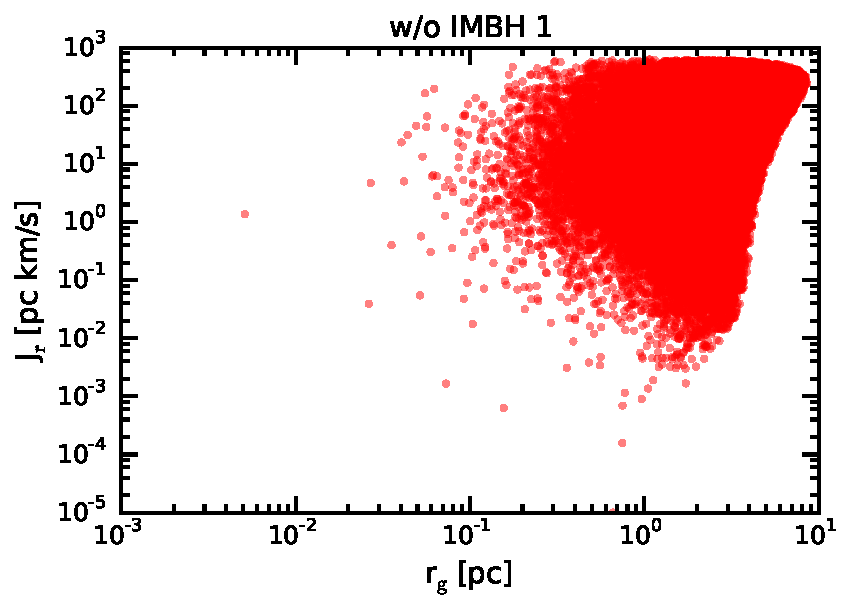
\includegraphics[width=\textwidth]{Plots/r_g_J_r_noIMBH1.png}
		\caption{SIM 3}
		\label{fig:r_g_J_r_noIMBH1}
	\end{subfigure}
	\hfill
	\begin{subfigure}{0.475\textwidth}
		\centering
		\includegraphics[width=\textwidth]{Plots/r_g_J_r_noIMBH2.png}
		\caption{SIM 4}
		\label{fig:r_g_J_r_noIMBH2}
	\end{subfigure}
	\caption{Radial action over guiding-star radius with marked specific stars on a double logarithmic scale. The colors are given as in Figure \ref{fig:vel_disp}. All simulations have a similar shaped distributions except for the marked stars which are the ones belonging to group 1 and 2 (see Figure \ref{fig:E_J_r_hist}). The \acp{GC} without \ac{IMBH} have almost no stars below \unit[0.1]{pc}, while the other simulations go down until \unit[$10^{-5}$]{pc} including the stars of group 1. There is a gap in SIM 1 and SIM 2 from about 10 to \unit[20]{pc}. Due to this high distances this gap is most likely not a signature of the \ac{IMBH} but probably due to numerical inaccuracies.}
	\label{fig:r_g_J_r}
\end{figure}
In Figure \ref{fig:r_g_J_r}, the radial actions are plotted over their guiding-star distances. We highlight the stars of group 1 and group 2 taken from Figure \ref{fig:E_J_r_hist} for SIM 1 and SIM 2. In general, there are several stars which have a really small guiding-star radius (up to  \unit[\(10^{-5}\)]{pc}). In SIM 3 and SIM 4 only very few stars go below \unit[0.1]{pc}. We see a round border of the shape given by stars of group 1. It is really clear to see but only if we know which stars we have to select. We cannot draw this conclusion the other way around, i.e. selecting these star in this plot and select them in Figure \ref{fig:E_J_r_hist}. The sharp signatures in Figures \ref{fig:r_g_J_r_IMBH1} and \ref{fig:r_g_J_r_IMBH2} at large guiding-star radii are probably due to numerical issues with deriving the guiding-star radius. But they do not affect the conclusion about signatures of the \ac{IMBH}, as these stars are in general far away from the \ac{IMBH}.

